% !TEX encoding = UTF-8 Unicode
% !TEX TS-program = pdflatex
% !TEX spellcheck = en-US
% !TEX root = ../Report.tex

\chapter{Vehicle Simulator}

No simulation would be possible without a simulator to run on.
Actually, the quality of a simulator can greatly affect the reliability of the final results and the success of the whole design process.
Luckily, there is a tool right for this: the \textbf{\mwVDB\texttrademark}.

The \mwVDB{} is an add-on from \mwMW{} that provides a rich set of tools for advanced simulation of automotive sub-systems.
These range from detailed models for wheels, suspensions, gearboxes and engine types to full vehicle motion up to 14 degrees of freedom altogether.
Moreover, simulation can be run in fully featured 3D environments with real-time interaction, leveraging the well known \textbf{Unreal Engine 4}.

In order to take advantage of such a game-changer and ensure the most realistic simulation possible,
we re-casted all the initial code to a \mwSL{} project and integrated it with these new components.


	\section{Simulation Environment}

	The \mwVDB{} offers a set of ready-made scenarios implementing standard maneuvers, from a simple sweept steer to obstacle avoidance according to ISO 3888-2.
	These scenarios, called \emph{Reference Applications}, share a common \mwSL{} project with convoluted scripting behind the scenes, to ensure proper settings
	when switching maneuvers. Furthermore, each subsystem provides different variants that allows for different interchangeable car types, components and environmental
	conditions to be easily selected through the \emph{Variant Manager}.
	\begin{center}
		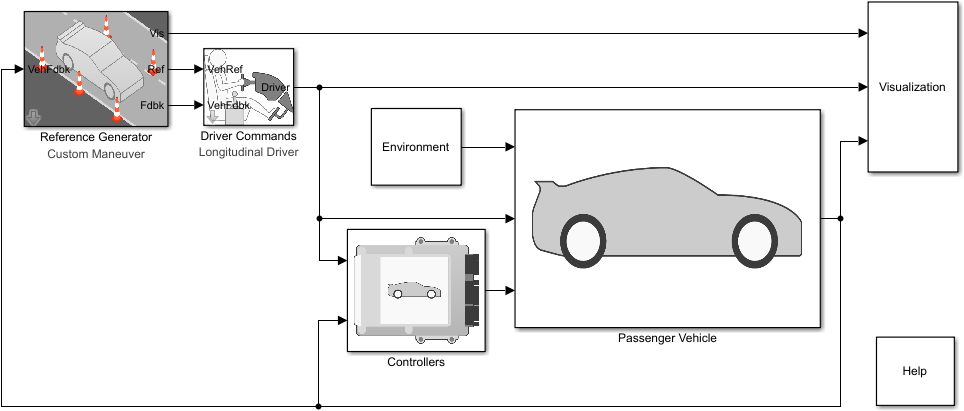
\includegraphics[width=0.9\textwidth]{Images/Simulator/sim-full}
	\end{center}


		\subsection{Passenger Vehicle}
		\label{ssec:vs-env-passveh}

		The core of the simulator resides inside the \emph{Passenger Vehicle} block.
		Besides the simple look of the cover image, this subsystem is a fine-grained model of a passenger car that reproduces not only the motion of a body in a 3D world,
		but every dynamic behavior of typical vehicle subsystems.

		The whole model is divided in two main sub-blocks. The \emph{Body} sub-block models the behavior of the unpowered chassis, in particular the suspension-road-tires
		interaction, extracting the resultant forces acting on the body given the drive torque. These forces are then processed by the \emph{Vehicle Body 3DOF} block to
		update the course taking into account additional phenomena including wind conditions, road incline and friction coefficients for each wheel (these two can be even
		extracted from real-time interaction with the 3D environment).

		The Body sub-system works on pure force and torque inputs, which are primarily provided by the second main piece: the \emph{Driveline}.
		This part translates typical controls available to a human driver into final wheel drive torques and brake commands by simulating the whole powertrain.
		It features both spark- and compression-ignition engines with mapped cycles, a fixed gear transmission and various differential flavors, all selected through variants.
		It also models the steering mechanism from driver to the wheels according to three different schemes, namely \emph{Parallel}, \emph{Rack-and-Pinion} and
		\emph{Ackerman}.

		The remaining sub-blocks are just signal pass-through boxes that route monolithic, high-level busses to their corresponding I/O ports. As such, these formal subsystems
		are of little functional significance and quite self explanatory.


		\subsection{Controllers}

		In the \emph{Controller} block are housed all the typical electronic control units found on modern cars. The most typical one is the \emph{Anti-lock Braking System},
		but there are also the differential control and others.
		\begin{center}
			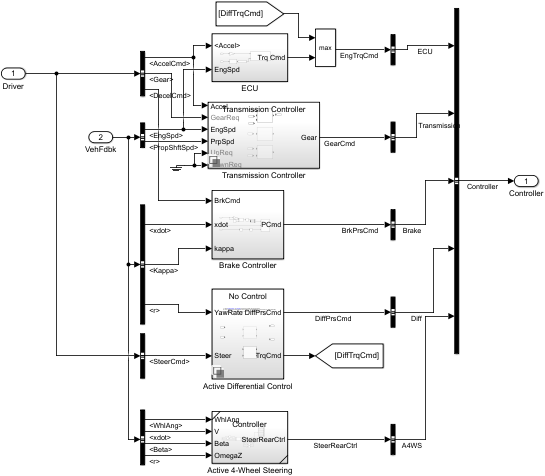
\includegraphics[width=0.9\textwidth]{Images/Simulator/ctrl-full}
		\end{center}

		Even though physically separated from the rest of the vehicle model, it is tightly coupled with that one, as it would be in the real world. As said before, any of these ECUs
		can be enabled through the corresponding variants.

		\subsection{Driver}
		\label{ssec:vs-env-drv}

		The \emph{Driver} block does exactly what it says, it drives the vehicle according to a provided reference path.
		The available variants include a \emph{Predictive Driver} that follows a path by acting on both the speed commands and the steering wheel,
		a \emph{Longitudinal Driver} for speed profiles only and an \emph{Open-Loop Driver} which basically passes on external, raw commands to the vehicle
		while maintaining consistency with the signal interface.

		This is somehow the most enigmatic of the blocks, mostly in lateral driving situations. Our understanding is that the Predictiove Driver was designed only for
		lateral displacement driving actions like in lane change maneuvers. However, the \emph{Constant Radius} reference application features an active curved-trajectory
		scenario where the Predictive Driver is employed through a mangling of the feedback signals from the vehicle, tricking the driver into a sort of constant lane change. As
		we'll better explain in~\vref{ssec:vs-int-cm}, the complex algorithm for predictive driving often reached an unstable situation, jeopardizing any good result in our work.


		\subsection{Reference Generator}

		Here is where the director leads the orchestra. Despite the humble name, the \emph{Reference Generator} does much more than simply provide the reference path
		to the driver. It actually offers the main settings panel for selecting the type of maneuver, the 3D scenario and the simulated vehicle model, the cruise speed and specific
		maneuver parameters. In the background, each callback to the scripts changes accordingly the remaining blocks of the simulator to meet the requests.
		\begin{center}
			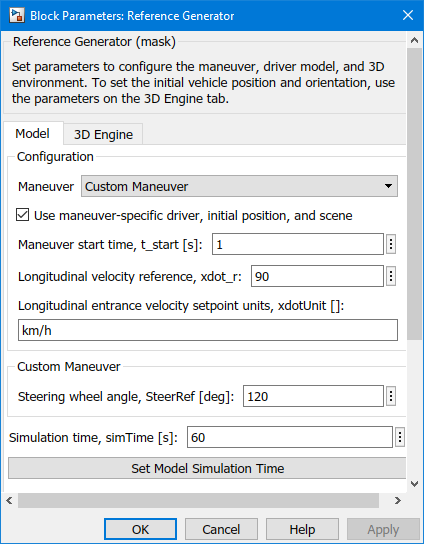
\includegraphics[height=0.3\textheight]{Images/Simulator/sim-refgen-cfg}
		\end{center}


		\subsection{Visualizer}

		The last component of the simulator is the \emph{Visualizer}, the most user-friendly of them all. Apart from collecting each and every useful signal from the whole system,
		the Visualizer offers a real-time dashboard showing the state of the car.
		\begin{figure}
			\centering
			\subfloat[][]{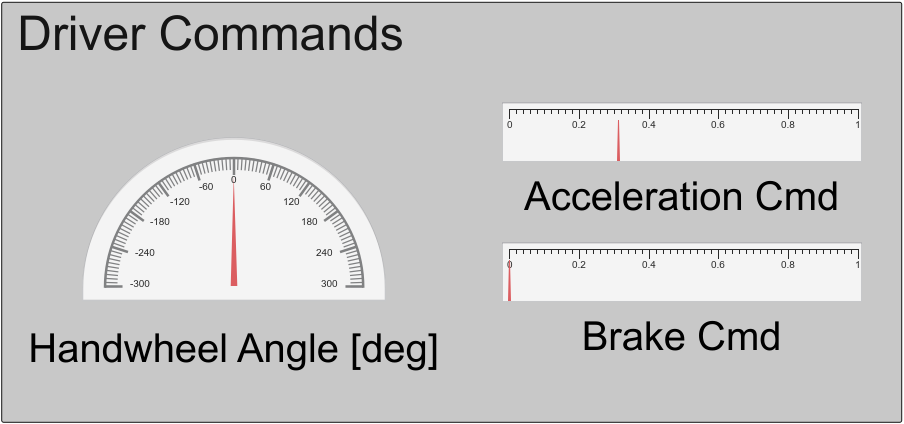
\includegraphics[height=0.12\textheight]{Images/Simulator/vis-dash-drv}}\quad
			\subfloat[][]{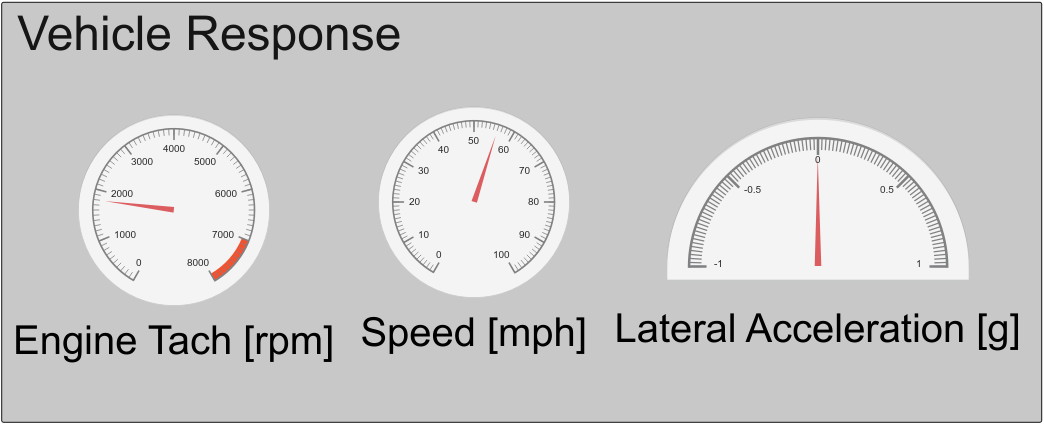
\includegraphics[height=0.12\textheight]{Images/Simulator/vis-dash-veh}}
			\caption{Detail of the real-time dashboard}
			\label{fig:vis-dash}
		\end{figure}
%		\begin{figure}
%			\centering
%			\subfloat[][]{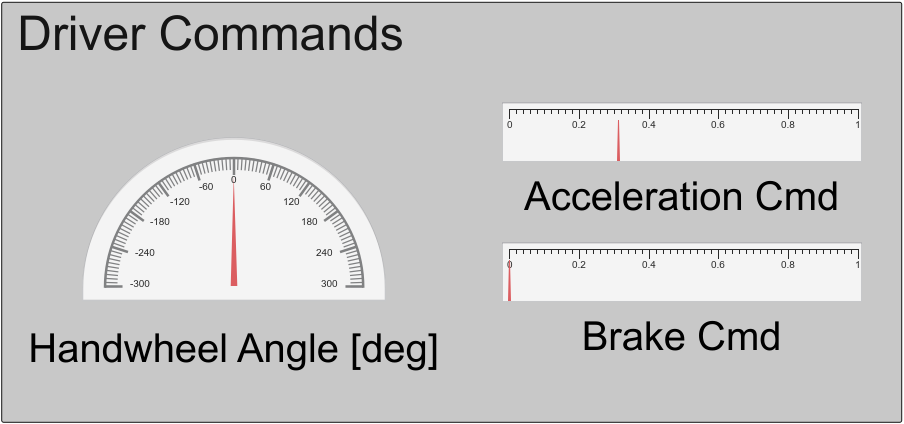
\includegraphics[width=0.45\textwidth]{Images/Simulator/vis-dash-drv}}\\
%			\subfloat[][]{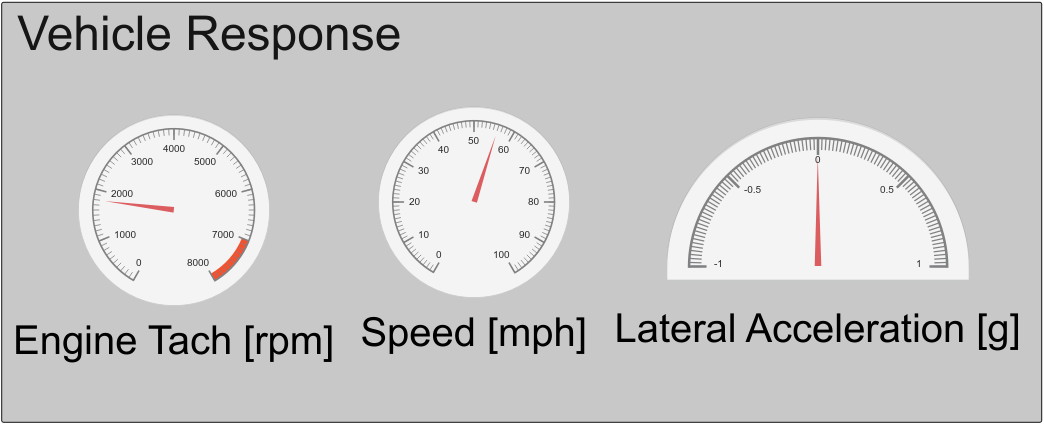
\includegraphics[width=0.45\textwidth]{Images/Simulator/vis-dash-veh}}
%		\caption{Detail of the real-time dashboard}
%		\label{fig:vis-dash}
%		\end{figure}

		It also implements all the machinery required to interface with the Unreal Engine 4 for realistic
		3D visualization of the whole action.


	\section{Integration}

	The framework described so far makes for a very flexible environment, yet it hardly satisfies our requirements out of the box.
	Yet, we wanted to preserve as much of the original functions as possible, with targeted inclusions rather than outright changes, sticking to the original structure and layout.
%	To blend seamlessly in such a sophisticated system, we performed some important changes in key components following the logical partitioning as much as possible.
	The first step to keep the reference application clean is to reference its project file from within ours. This technicality boils down to a \mwSL{} model with a single block
	referencing to the simulator top-level model, to establish the dependency. For all the other development purposes, \texttt{model/A4WS.slx} is a mere placeholder and the
	\lstinline{CRReferenceApplication} block should be opened as the top-level model each time through the dedicated button in the bottom-left corner.


		\subsection{Rear Steering}

		First and foremost, we needed a rear-steered car. Since an active rear-steering control is still uncommon, the original simulator had no variant for that and required some
		\mwSL{} plumbing. Nonetheless, the Passenger Vehicle~\ref{ssec:vs-env-passveh} subsystem follows a redundant but consistent structure and provides a signal bus
		for all four wheel angles, among others. This helped a lot, since we just had to arrange a dedicated \emph{Kinematic Steering} for the rear wheels inside the
		\emph{Driveline}, replace the grounded wheel signal with its output and finally route the input up to our control unit (see below), following all translation stages and bus
		aggregations.
		\begin{figure}
			\centering
			\subfloat[][Rear Steering signal routing]{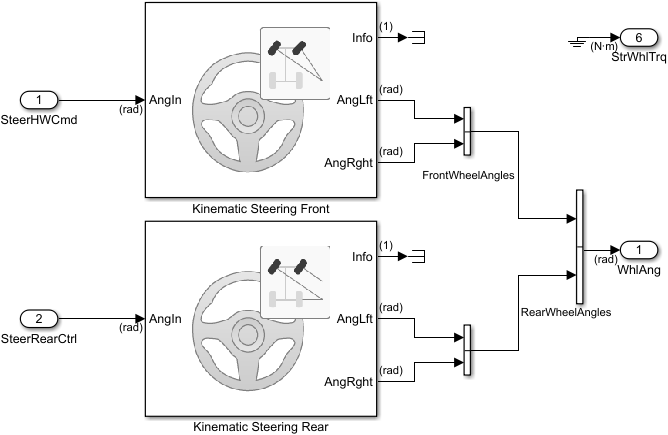
\includegraphics[width=0.45\textwidth]{Images/Simulator/veh-drvln-steer}}\quad
			\subfloat[][Body model adaptation]{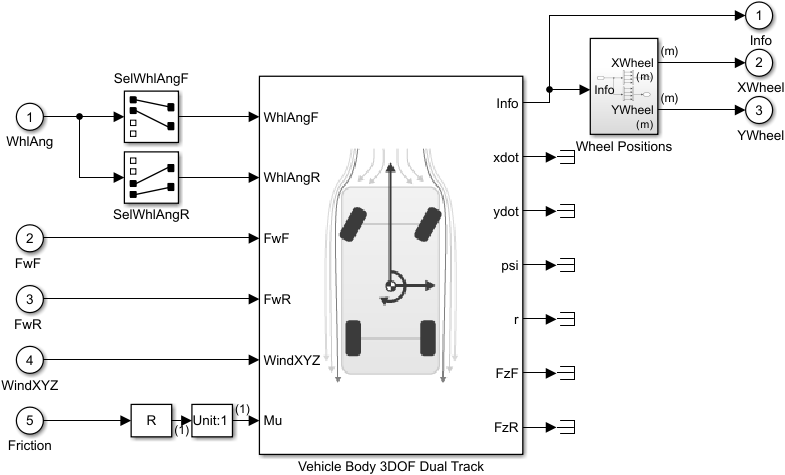
\includegraphics[width=0.45\textwidth]{Images/Simulator/veh-body-detail}}
			\caption{}
			\label{}
		\end{figure}

		The Kinematic Steering for the rear wheels is set to a ratio of 1:1 for direct wheel control, while saturating the maximum steering range according to the
		\lstinline{rngRearSteer} parameter in \texttt{model/SimRoutine.m} (the default range is $\pm\ang{5}$). A counterintuitive setting is the \emph{Front} option,
		which ensures the wheels get the angle signal of the same sign as the control output.


		\subsection{A4WS Control Unit}
		\label{ssec:vs-int-ctrl}

		Consistent with the overall layout, our \emph{\awwwws} control unit is located inside the Controllers block with all the other ECUs.
		Basically, it is a separate \mwSL{} sub-model inside \texttt{model/Controller.slx} enclosing our development into a separate container, for better abstraction.
		The block taps into the vehicle \emph{feedback bus} to retrieve the required system data, namely \emph{speed}, the \emph{side-slip angle} and \emph{yaw rate},
		while the \emph{rear-steer angle} output is included in the \emph{Controller} bus with the dedicated \lstinline{A4WS/CmdRearSteer} channel and reaches the kinematic
		steering element in the driveline subsystem (see above).

		Inside \texttt{model/Controller.slx} the actual control block --- a \emph{\mwML{} Function} --- communicates with the outside world through two translation blocks.
		These subsystems take care of proper unit conversion and reference frame translation, as the whole simulator is built around a down-pointing frame, while we felt
		more comfortable with the usual choice of the Z axis pointing against gravity. Luckily, the signals involved include only yaw angles and changing the sign does the job.
		\begin{center}
			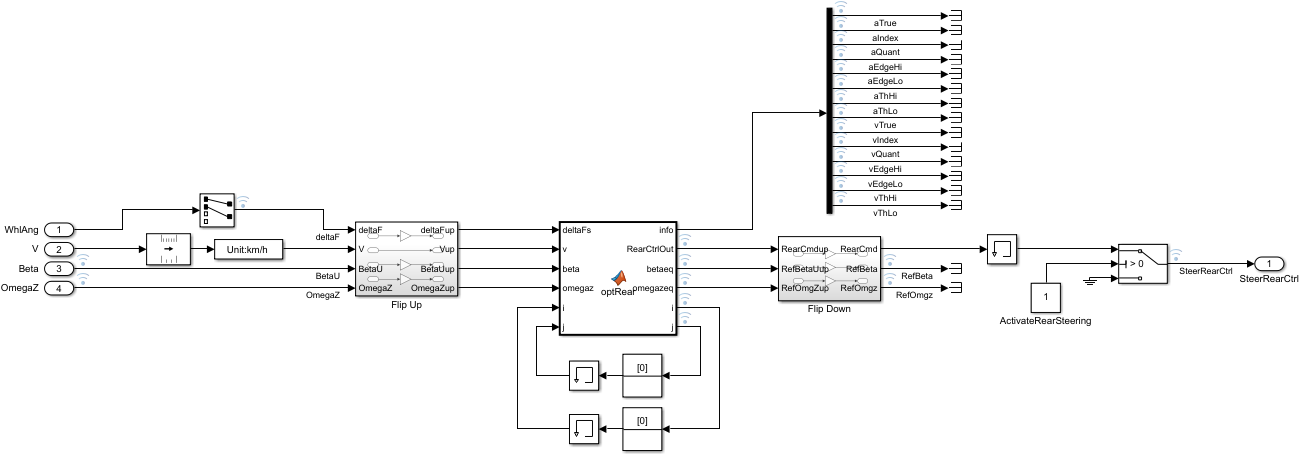
\includegraphics[width=0.9\textwidth]{Images/Simulator/a4ws-full}
		\end{center}

		The beefy part of the controller is inside the function block \lstinline{optRear} and, as the name suggests, it is where the state is fed back to the system scaled by a scale
		matrix, obtained through optimal control as described in \vref{sec:vs-ctrl}. Prior to this, two important action are performed.
		First, the right gain coefficients are picked from the look-up table \lstinline{Klut}, according to the mean-value of the current front wheel angles and the speed.
		To avoid harmful glitches, there is a hysteretic mechanism that switches to another gain matrix K only if the threshold has been crossed with enough margin.
		\lstinputlisting[firstline=7, lastline=41, firstnumber=7]{Images/Simulator/a4ws-code.m}
		The inner workings of this selection process are made available at the \lstinline{info} port and features two sets of seven values for the true value, the quantized one,
		the would-be index and the upper and lower values for both the division boundaries and the thresholds.
		\lstinputlisting[firstline=43, lastline=43, firstnumber=43]{Images/Simulator/a4ws-code.m}

		The settings for these threshold, expressed in percentage over one division of the full range, can be found at the very beginning of \texttt{model/SimRoutine.m}:
		\lstinputlisting[firstline=24, lastline=30, firstnumber=24]{../../../model/SimRoutine.m}

		The second step is to extract the instantaneous equilibrium point by inverting on-the-fly the matrix $A$, to adapt the reference signals to external conditions as well:
		\lstinputlisting[firstline=46, lastline=86, firstnumber=46]{Images/Simulator/a4ws-code.m}

		Once the controller have all the ingredients ready, the usual operation $u = -Kx$ is performed and returned at the output:
		\lstinputlisting[firstline=90, firstnumber=90]{Images/Simulator/a4ws-code.m}


		\subsection{Custom Maneuver}
		\label{ssec:vs-int-cm}

		Unfortunately, the provided scenarios where difficult to use out-of-the-box, so instead of radically changing them we decided to add our custom maneuver.
		It might seem a straightforward approach, yet there are a fair amount of cross-scripts to take care of to make the new scenario fit in the simulator.
		By examining the \emph{mask layout} of the Reference Generator block, we were able to track all the script involved and mirror the required actions on our case.

		Most notably, we choose to set the Driver to a Longitudinal one and provide direct signals for the steering wheel. The initial hype for the Predictive Driver faded as
		we experienced more and more instability during early simulations. The algorithm implemented in such advanced driver model was hard to interpret and fix, so we traded
		off some realism for quicker results. Moreover, the block is intended for lateral references along a straight path, like lane-change maneuvers on a highway.
		As mentioned in \vref{ssec:vs-env-drv}, the \emph{Constant Radius} maneuver uses a Predictive Driver to achieve a circular path, by overriding the feedback signals
		from the vehicle and tricking the driver into perceiving the car on a straight road and feeding back the turn reference as a constant displacement from the centerline.

		Once the Predictive Driver got discarded, we moved on to implement our reference maneuvers. Again, we took advantage of \mwSL{} model variants to create a set of
		simple patterns, yet perfectly repeatable and simple to interpret. They sum up to:
		\begin{description}

			\item[Constant] The steering wheel is kept constant for the whole time;

			\item[2-Step] The steering wheel briefly steps to the given angle a quickly settles to its double for the rest of the time;

			\item[Lane-Change] The vehicle is steered first to the given direction, then straightened up and finally steered back to the starting lane after ten seconds;

			\item[Evasive] Similar to the lane-change maneuver, but reverts to the original lane much quicker, similarly to an obstacle avoidance action.

		\end{description}

		Each maneuver is initiated at time \SI{20}{\second} and both the \emph{speed} and \emph{steering wheel angle} are set in the Reference Generator settings dialog.
		The time delay is to let the speed build up before system excitation. For the more articulated maneuvers, the steering profile is obtained by a chain of step generators
		compensating each other at different time steps. It's a crude yet effective way to lay a pattern and despite the unrealistic step variation of the steering, this ensures that
		good results could only improve with smoother excitation.
		\begin{center}
			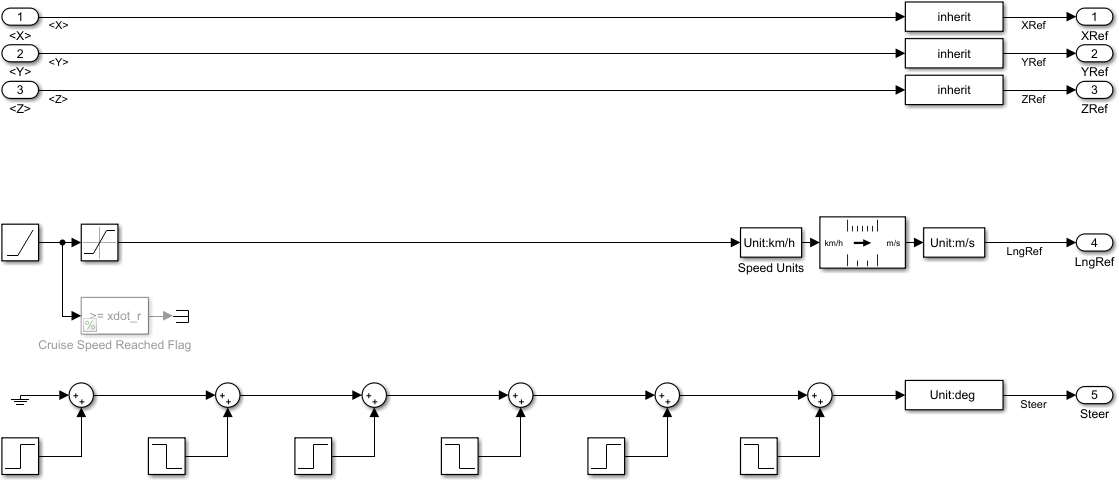
\includegraphics[width=0.9\textwidth]{Images/Simulator/cm-s-full}
		\end{center}


		\subsection{Environment}

		In a very similar way to the steering patterns in the previous section, we implemented also a set of adverse environmental conditions.
		Even if logically implemented in distinct sub-blocks, we list them altogether:
		\begin{description}

			\item[No Wind] The aerodynamic force is completely suppressed;

			\item[Lateral] The vehicle is subject to a constant wind, blowing in the negative lateral direction;

			\item[Burst] Same as Lateral wind, except the vehicle experiences a brief burst of wind;

			\item[Ideal Road] The road presents a unit scaling factor for the tire friction force;

			\item[Ice Patch] The car travels through an icy patch and then recovers traction;

			\item[Snowy Range] The road switches from tarmac to snow for the rest of the time.

		\end{description}

		Again, these disturbances kick in few seconds after the maneuver is initiated, to let the vehicle build up some spin and make the effect more dramatic.
		As usual, model variants lets the two phenomena combine together at will.
		\begin{figure}
			\centering
			\subfloat[][\lstinline{Environment} block]{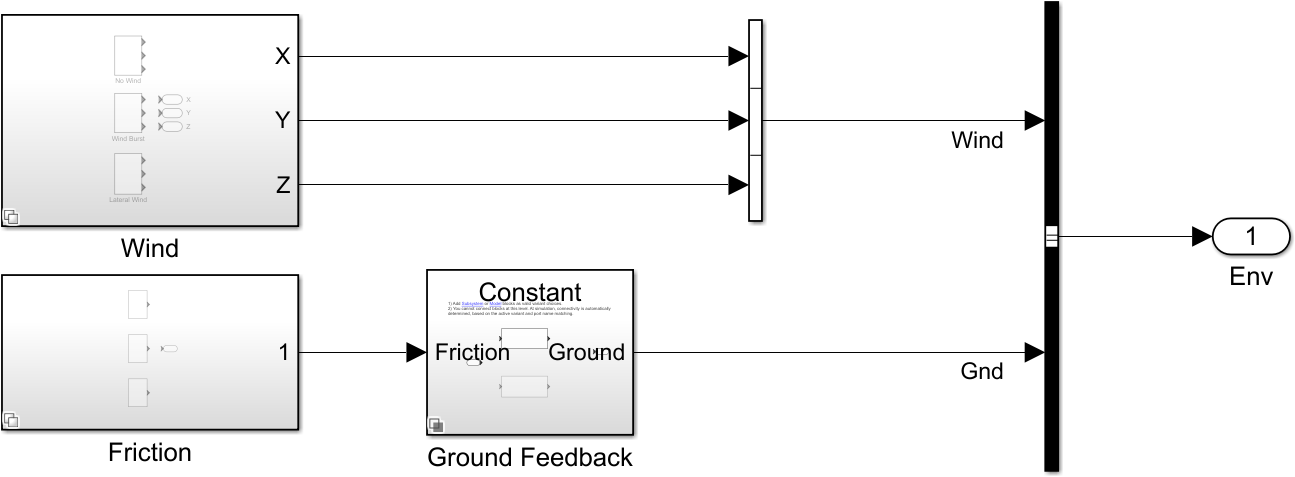
\includegraphics[width=0.55\textwidth]{Images/Simulator/env-full}}\quad
			\subfloat[][\lstinline{Wind Burst} sub-block]{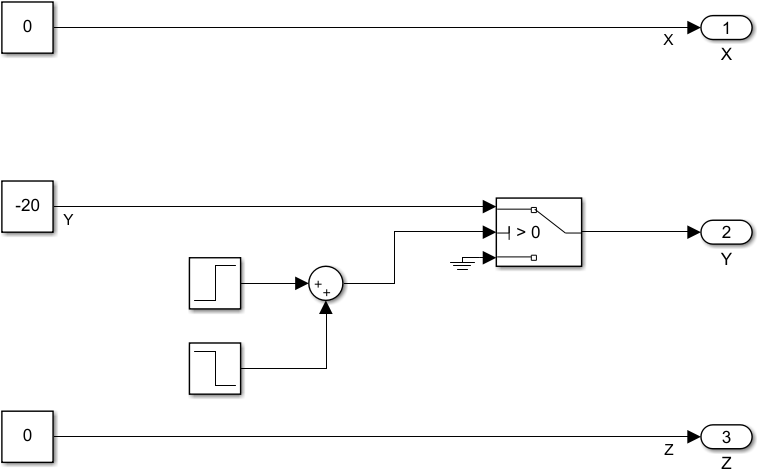
\includegraphics[width=0.35\textwidth]{Images/Simulator/env-wind-burst}}
			\caption{}
			\label{}
		\end{figure}


	\section{Control}
	\label{sec:vs-ctrl}

	The last, crucial component that completes our project is a set of scripts that perform calculus and drive the simulator to obtain the resulting data.
	The entry point for the whole simulation is \texttt{model/SimScript.m}, which first extracts vehicle parameters from the model workspace and sets some constants for the size and
	the resolution of the control look-up tables (as seen in \ref{ssec:vs-int-ctrl}):
	\lstinputlisting[firstline=22, lastline=34, firstnumber=22]{../../../model/SimRoutine.m}
	Then, it hands all the parameters to the optimization engine:
	\lstinputlisting[firstline=36, lastline=37, firstnumber=36]{../../../model/SimRoutine.m}
	Finally, the simulation sequence is launched:
	\lstinputlisting[firstline=40, lastline=44, firstnumber=40]{../../../model/SimRoutine.m}
	The rest of the code formats the output data and plots the results. Its expansion \texttt{model/SimRoutine2.m} automates the simulation for different environmental conditions.

	The optimization engine takes an intermediate step inside \texttt{model/LUTScript.m}, which populates the look-up table used by the controller with the gain coefficients.
	These are obtained from subsequent invocations of \texttt{model/LinPlant.m}:
	\lstinputlisting[firstline=16, firstnumber=16]{../../../model/LUTScript.m}
	Here the vehicle body dynamics are linearized around the provided point and control law
	parameters are calculated through \emph{Optimal Control} methods, namely the \lstinline{lqr} \mwML{} function.
